%----------------------------------------------------------------------------------------
% mhd_bperp.tex
% evolution of tangential magnetic field 
%----------------------------------------------------------------------------------------
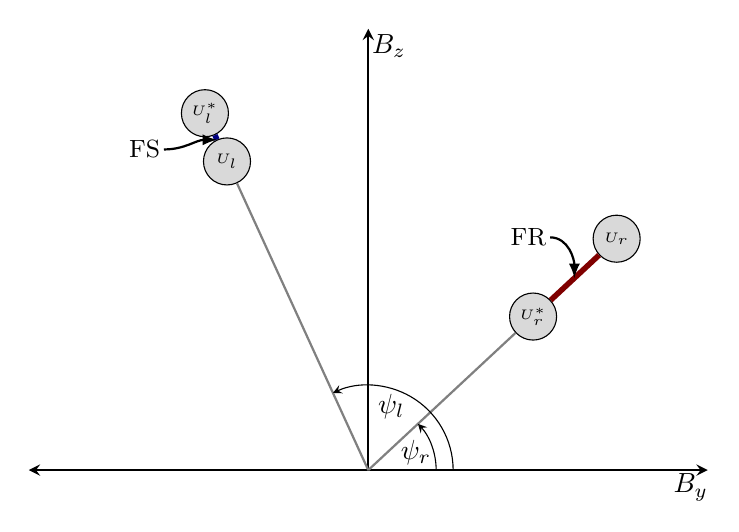
\begin{tikzpicture}[scale = {0.0125\linewidth},
    >=stealth, %
    inner sep=1pt, %outer sep=2pt,%
    axis/.style={thick,->},
    base node/.style={circle,draw,minimum size=17pt}]

  % axis
  \draw[thick] (0.95,0) node[below]{$B_y$}-|(0,1.25) node[right]{$B_z$};
  \draw[axis] (0.95,0)--(1.0,0);
  \draw[axis] (0,1.25)--(0,1.3);  
  \draw[axis] (0,0)--(-1,0);

  % Colors
  \colorlet{darkblue}{blue!50!black}
  \colorlet{darkred}{red!50!black}

  %---------------------------------------------
  % connect rotations
  %---------------------------------------------
  %% \draw[-,darkred, line width = 2pt] ++(42.972:0.66359) arc(42.972:90.232:0.66359);
  %% \draw[-,darkblue, line width = 2pt]++(114.59:1.15621)arc(114.592:90.232:1.15621);

  %---------------------------------------------
  % place node corresponding to shapes
  %---------------------------------------------
  \node[base node,draw,shape=circle,fill=gray!30] (R8) at (114.592:1.0) {\tiny $\mbf{U}_{l}$};
  \node[base node,draw,shape=circle,fill=gray!30] (R7) at (114.592:1.15621) {\tiny $\mbf{U}^*_{l}$};
  %% \node[base node,draw,shape=circle,fill=gray!30] (R6) at (90.232:1.15621) {\tiny $\mbf{U}^*_{2r}$};
  %% \node[base node,draw,shape=circle,fill=gray!30] (CD) at (90.232:0.84200) {\tiny CD};
  %% \node[base node,draw,shape=circle,fill=gray!30] (R3) at (90.232:0.66359) {\tiny $\mbf{U}^*_{2l}$};
  \node[base node,draw,shape=circle,fill=gray!30] (R2) at (42.972:0.66359) {\tiny $\mbf{U}^*_{r}$};
  \node[base node,draw,shape=circle,fill=gray!30] (R1) at (42.972:1.0) {\tiny $\mbf{U}_{r}$};

  %---------------------------------------------
  % connect nodes
  %---------------------------------------------
  \draw[gray,thick](0:0) -- (R2);
  \draw[darkred, line width = 2pt](R1) -- (R2);
  %% \draw[darkred, line width = 2pt](R3) -- (CD);
  %% \draw[darkblue, line width = 2pt](CD) -- (R6);
  \draw[darkblue, line width = 2pt](R7) -- (R8);
  \draw[gray,thick](0:0) -- (R8);
  
  %---------------------------------------------
  % place node corresponding to shapes
  %---------------------------------------------
  \path (0,0)++(70:0.2)node{$\psi_l$};
  \draw[->](0:0.25)arc(0:114.592:0.25);

  \draw[->](0:0.2)arc(0:42.972:0.2);
  \path (0,0)++(20:0.15)node{$\psi_r$};
  
  \draw[-latex,thick](122.5:1.12)node[left]{\small FS}
  to[out=0,in=180] (114.592:1.07);
  
  %% \draw[-latex,thick](97.5:1.25)node[right]{\small RD}
  %% to[out=180,in=90] (102:1.15621);
  
  %% \draw[-latex,thick](97.5:1.0)node[left]{\small SS}
  %% to[out=0,in=180] (90.232:1.0);
  
  %% %% \draw[-latex,thick](0.61,0.40)node[right]{\small CD}
  %% %% to[out=180,in=0] (0.51,0.45);
  
  %% \draw[-latex,thick](80.5:0.775)node[right]{\small SR}
  %% to[out=180,in=0] (90.232:0.75);
  
  %% \draw[-latex,thick](70:0.55)node[left]{\small RD}
  %% to[out=0,in=270] (66.0:0.66359);
  
  \draw[-latex,thick](52:0.87)node[left]{\small FR}
  to[out=0,in=90] (42.972:0.83);

\end{tikzpicture}
